\section{Suppose that two random variables
\texorpdfstring{$X_1$}{X1} and \texorpdfstring{$X_2$}{X2} have
a continuous joint distribution for which the joint PDF is as follows: 
\texorpdfstring{$f(x_1, x_2) = 4x_1x_2$ for $0<x_1<1$ and $0<x_2<1$,
$=0$ otherwise}{f(x1, x2) = 4x1x2 for 0<x1<1 and 0<x2<1, =0 otherwise}.
Now consider the change of variables 
\texorpdfstring{$Y_1 = X_1 / X_2, Y_2 = X_1 X_2$}{Y1 = X1 / X2, Y2 = X1 X2},
and let \texorpdfstring{$g(y_1, y_2)$}{g(y1, y2)} be the joint PDF of these two
variables. Sketch the region in the \texorpdfstring{$y_1, y_2$}{y1, y2} plane
for which \texorpdfstring{$g$}{g} is non-zero, and calculate
\texorpdfstring{$g(y_1, y_2)$}{g(y1, y2)}.}

To sketch the region, first notice the possible ranges of the variables.

$y_1$ can take any value between 0 and infinity. $y_2$ has a lower bound of zero and a global upper bound of 1.

But consider minimum and maximum values of $y_2$ for a given $y_1$.

If $y_1 \leq 1$, our maximal value will be found by taking $x_2=1$ (well arbitrarily close to 1), which means $y_1 = x_1$ which in turn means $y_2 = y_1$ (again in the same arbitrarily close way). 

On the other hand if $y_1 > 1$, we can find the value by taking $x_1=1 \implies y_2 = x_2 \implies y_2 = \frac{1}{y_1}$.

A sketch of the region where $g \neq 0$ is as follows:
\begin{figure*}[h]
    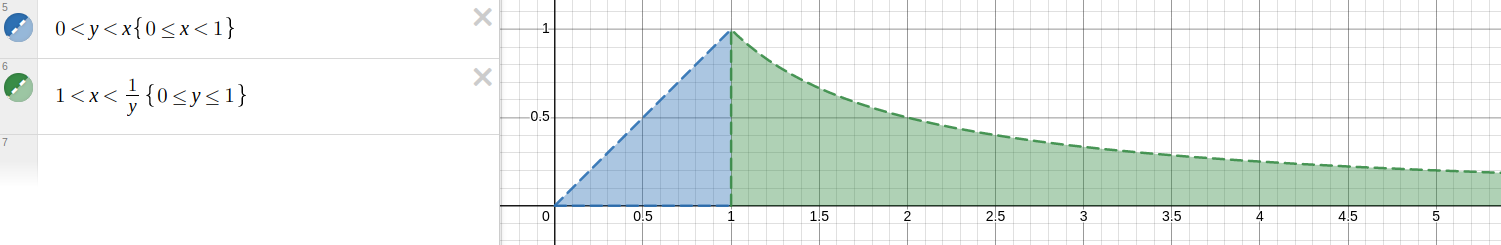
\includegraphics[width=\textwidth]{q4_region.png}
\end{figure*}

To find $g(y_1, y_2)$ use the Jacobian:

\begin{align*}
    g(y_1, y_2) &= f(x_1, x_2) \left|\begin{matrix}
        \frac{\partial x_1}{\partial y_1} & \frac{\partial x_1}{\partial y_2} \\
        \frac{\partial x_2}{\partial y_1} & \frac{\partial x_2}{\partial y_2} \\
    \end{matrix}\right| \\
\end{align*}

To find these, we'll need $x_1(y_1, y_2), x_2(y_1, y_2)$:
\begin{align*}
    y_1 &= \frac{x_1}{x_2} \\
    y_2 &= x_1x_2 \implies x_2 = \frac{y_2}{x_1}\\
    y_1 &= \frac{x_1}{\frac{y_2}{x_1}} \\
    \implies x_1^2 &= y_1y_2 \\
    x_1 &= \sqrt{y_1y_2} \\
    x_2 &= \sqrt{\frac{y_2}{y_1}} \\
\end{align*}

\begin{align*}
    g(y_1, y_2) &= 4x_1x_2 \left|\begin{matrix}
        \frac{1}{2}\sqrt{\frac{y_2}{y_1}} & \frac{1}{2}\sqrt{\frac{y_1}{y_2}} \\
        -\frac{1}{2}\sqrt{\frac{y_2}{y_1}}\frac{1}{y_1} & \frac{1}{2}\sqrt{\frac{1}{y_1y_2}} \\
    \end{matrix}\right| \\
    &= 4y_2 \left|
        \frac{1}{2}\sqrt{\frac{y_2}{y_1}}
        \frac{1}{2}\sqrt{\frac{1}{y_1y_2}} + 
        \frac{1}{2}\sqrt{\frac{y_1}{y_2}} 
        \frac{1}{2}\sqrt{\frac{y_2}{y_1}}\frac{1}{y_1}
    \right| \\
    &= 4y_2 \left(
        \frac{1}{4y_1} + 
        \frac{1}{4y_1}
    \right) \\
    &= \frac{2y_2}{y_1} \\
\end{align*}
